
% This LaTeX was auto-generated from an M-file by MATLAB.
% To make changes, update the M-file and republish this document.

\documentclass{article}
\usepackage{graphicx}
\usepackage{color}

\sloppy
\definecolor{lightgray}{gray}{0.5}
\setlength{\parindent}{0pt}

\begin{document}

    
    
\section*{Measuring and Modelling Evapotranspiration}

\begin{par}
Authors:       Debora J�ckel, Simon Roth, Gabriela Sch�r, Alexandra Schuler //                Institute of Environmental Engineering, ETH Zurich //                Labor II // Version:       March 2013 // Last revision: 20. March 2013
\end{par} \vspace{1em}

\subsection*{Contents}

\begin{itemize}
\setlength{\itemsep}{-1ex}
   \item Reset workspace
   \item Import data
   \item Analysis specification
   \item Define constants
   \item Define vectors
   \item Compute evapotranspiration
   \item Figures
   \item Free memory
\end{itemize}


\subsection*{Reset workspace}

\begin{verbatim}
clear all
close all
\end{verbatim}


\subsection*{Import data}

\begin{verbatim}
lysimeter.folder = 'data/2012/lysimeter/';
lysimeter.file   = '2012_lysimeter_01.txt';
meteo.folder     = 'data/2012/meteo/';
meteo.file       = '2012_meteodata_data.txt';

% read data
lysimeter.data = dlmread( [ lysimeter.folder lysimeter.file ] );
meteo.data     = dlmread( [ meteo.folder meteo.file ], ';', 3, 1 );

% correct time shift
lysimeter.data( :, 1 ) = datenum( num2str( lysimeter.data( :, 1 ) ), 'yyyymmddHH' );
meteo.data             = [ nan( 1, size( meteo.data, 2 ) ); meteo.data ];
meteo.data             = [ lysimeter.data( :, 1 ), meteo.data( 1:end-1, 2:end ) ];
\end{verbatim}


\subsection*{Analysis specification}

\begin{verbatim}
t          = { '01.01.2012', '31.12.2012' };	% [dd.mm.yyyy]
plant      = 'Raps';
cropFactor = 1.15;                              % [-]
\end{verbatim}


\subsection*{Define constants}

\begin{verbatim}
alpha    = 0.23;            % [-]
latitude = 47+26/60;        % [�]
Gsc      = 0.0820;          % [MJ/m2 min]
hGeo     = 443;             % [m]
sigma    = 4.903*10^-9;     % [MJ/K4 m2 d]
\end{verbatim}


\subsection*{Define vectors}

\begin{verbatim}
% time
time.h = lysimeter.data( :, 1 );
time.d = floor( dailyMean( time.h ) );
time.m = datevec( floor( monthlyMean( time.h, time.h ) ) );
time.m = datenum( time.m )-time.m( :, 3 )+1;
time.y = year( mean( time.h ) );

% storage [mm]
storage.h = gradient( lysimeter.data( :, 4 ) );
storage.d = dailySum( storage.h );
storage.m = monthlySum( storage.h, time.h );

% percolation [mm]
percol.h = lysimeter.data( :, 5 );
percol.d = dailySum( percol.h );
percol.m = monthlySum( percol.h, time.h );

% solar radiation [W/m2]
Rs.h = meteo.data( :, 5 );
Rs.d = dailyMean( Rs.h );
Rs.m = monthlyMean( Rs.h, time.h );

% pressure [hPa]
press.h = meteo.data( :, 6 );
press.d = dailyMean( press.h );
press.m = monthlyMean( press.h, time.h );

% air temperature [�C]
Tair.h    = meteo.data( :, 7 );
Tair.dMax = dailyMax( Tair.h );
Tair.dMin = dailyMin( Tair.h );
Tair.d    = ( Tair.dMax+Tair.dMin )/2;
Tair.mMax = monthlyMean( Tair.dMax, time.d );
Tair.mMin = monthlyMean( Tair.dMin, time.d );
Tair.m    = ( Tair.mMax+Tair.mMin )/2;

% precipitation [mm]
percip.h = meteo.data( :, 9 );
percip.d = dailySum( percip.h );
percip.m = monthlySum( percip.h, time.h );

% relative humidity [%]
RH.h = meteo.data( :, 10 );
RH.d = dailyMean( RH.h );
RH.m = monthlyMean( RH.h, time.h );

% wind speed [m/s]
windSp.h = meteo.data( :, 12 );
windSp.d = dailyMean( windSp.h );
windSp.m = monthlyMean( windSp.h, time.h );

clear lysimeter meteo

% mean saturation vapour pressure [kPa]
es.d = ( satVapPressure( Tair.dMax )+satVapPressure( Tair.dMin ) )/2;
es.m = ( satVapPressure( Tair.mMax )+satVapPressure( Tair.mMin ) )/2;
\end{verbatim}


\subsection*{Compute evapotranspiration}

\begin{verbatim}
% actual evapotranspiration [mm]
AET.h = percip.h-percol.h-storage.h;
AET.d = percip.d-percol.d-storage.d;
AET.m = percip.m-percol.m-storage.m;

% Penman-Monteith [mm]
penMonPET.d = penmanMonteith( es.d, Tair.d, RH.d, alpha, Rs.d, time.d, latitude, Gsc, hGeo, sigma, Tair.dMax, Tair.dMin, press.d, windSp.d )*cropFactor;
penMonPET.m = penmanMonteith( es.m, Tair.m, RH.m, alpha, Rs.m, time.m, latitude, Gsc, hGeo, sigma, Tair.mMax, Tair.mMin, press.m, windSp.m )*cropFactor.*eomday( time.y, 1:12)';

% Turc [mm]
turcPET.d = turc( RH.d, Rs.d, Tair.d )*cropFactor;
turcPET.m = turc( RH.m, Rs.m, Tair.m )*cropFactor.*eomday( time.y, 1:12)';

% Ivanov [mm]
ivanovPET = ivanov( Tair, RH, cropFactor );

% Turc and Ivanov combined [mm]
turcIvanovPET.d = [ ivanovPET.d( 1:sum( eomday( time.y, 1:2 ) ) ); turcPET.d( sum( eomday( time.y, 1:2 ) )+1:sum( eomday( time.y, 1:10 ) ) ); ivanovPET.d( sum( eomday( time.y, 1:10 ) )+1:sum( eomday( time.y, 1:12 ) ) ) ];
turcIvanovPET.m = [ ivanovPET.m( 1:2 ); turcPET.m( 3:10 ); ivanovPET.m( 11:12 ) ];
\end{verbatim}


\subsection*{Figures}

\begin{par}
Instruction: niceFigure( time vector, [ all data vectors separated by commas ], \{ all labels for the data vector as strings separated by commas \}, the period, the titel of the plot )
\end{par} \vspace{1em}
\begin{verbatim}
niceFigure( time.d, [ AET.d, penMonPET.d ], { 'AET', 'Penman-Monteith' }, t, [ plant ' (daily)' ] )
niceFigure( time.m, [ AET.m, penMonPET.m ], { 'AET', 'Penman-Monteith' }, t, [ plant ' (monthly)' ] )
niceFigure( time.d, [ penMonPET.d, turcPET.d, ivanovPET.d, turcIvanovPET.d ], { 'Penman-Monteith', 'Turc', 'Ivanov', 'Turc and Ivanov combined' }, t, [ plant ' (daily)' ] )
niceFigure( time.m, [ penMonPET.m, turcPET.m, ivanovPET.m, turcIvanovPET.m ], { 'Penman-Monteith', 'Turc', 'Ivanov', 'Turc and Ivanov combined' }, t, [ plant ' (monthly)' ] )
\end{verbatim}

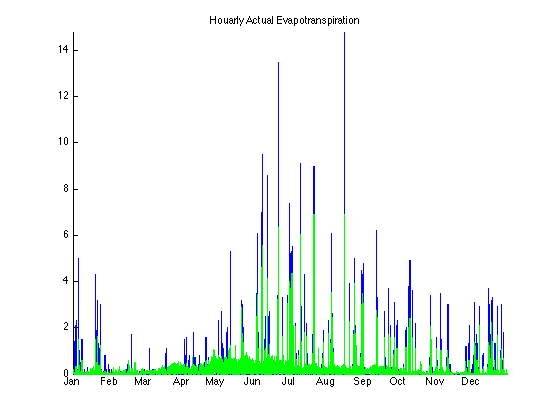
\includegraphics [width=4in]{main_01.eps}

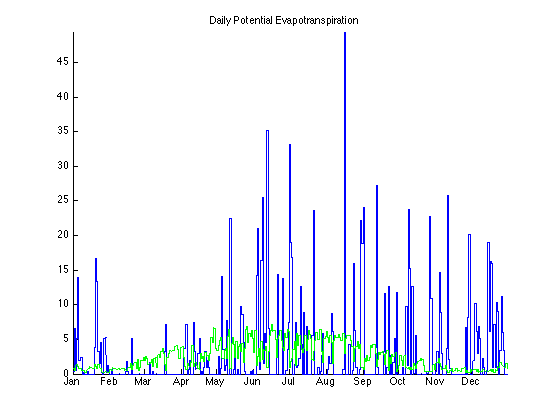
\includegraphics [width=4in]{main_02.eps}

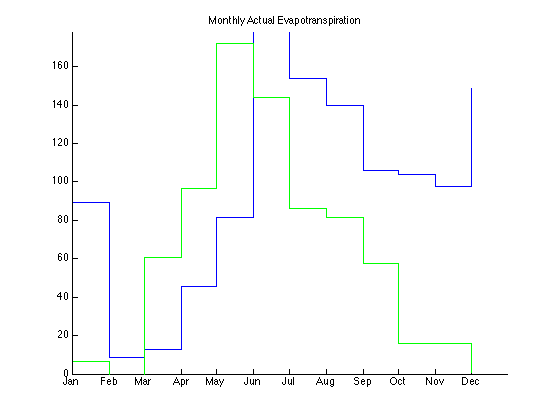
\includegraphics [width=4in]{main_03.eps}

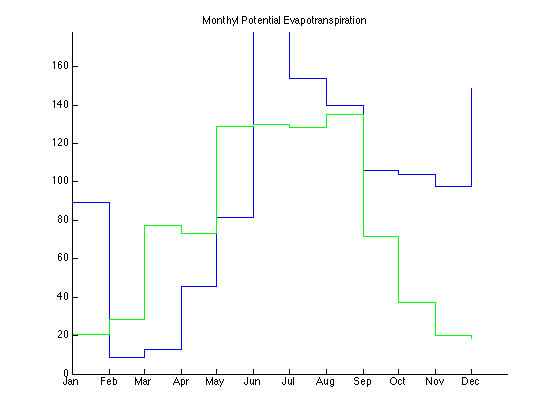
\includegraphics [width=4in]{main_04.eps}


\subsection*{Free memory}

\begin{verbatim}
clear all
\end{verbatim}



\end{document}
    
